\documentclass[12pt]{article}
\usepackage{enumerate}
\usepackage{mathematics}
\usepackage{oxford}

\newcommand{\Ch}{\mathcal{C}_h}

\begin{document}
\title{Oxford M1 - Groups and Group Actions \footnotetext{\url{https://courses.maths.ox.ac.uk/node/5552}}}
\author{}
\date{}
\maketitle

\section{Sheet 1: Binary Operations. The Group Axioms. Examples.}

\begin{mdframed}
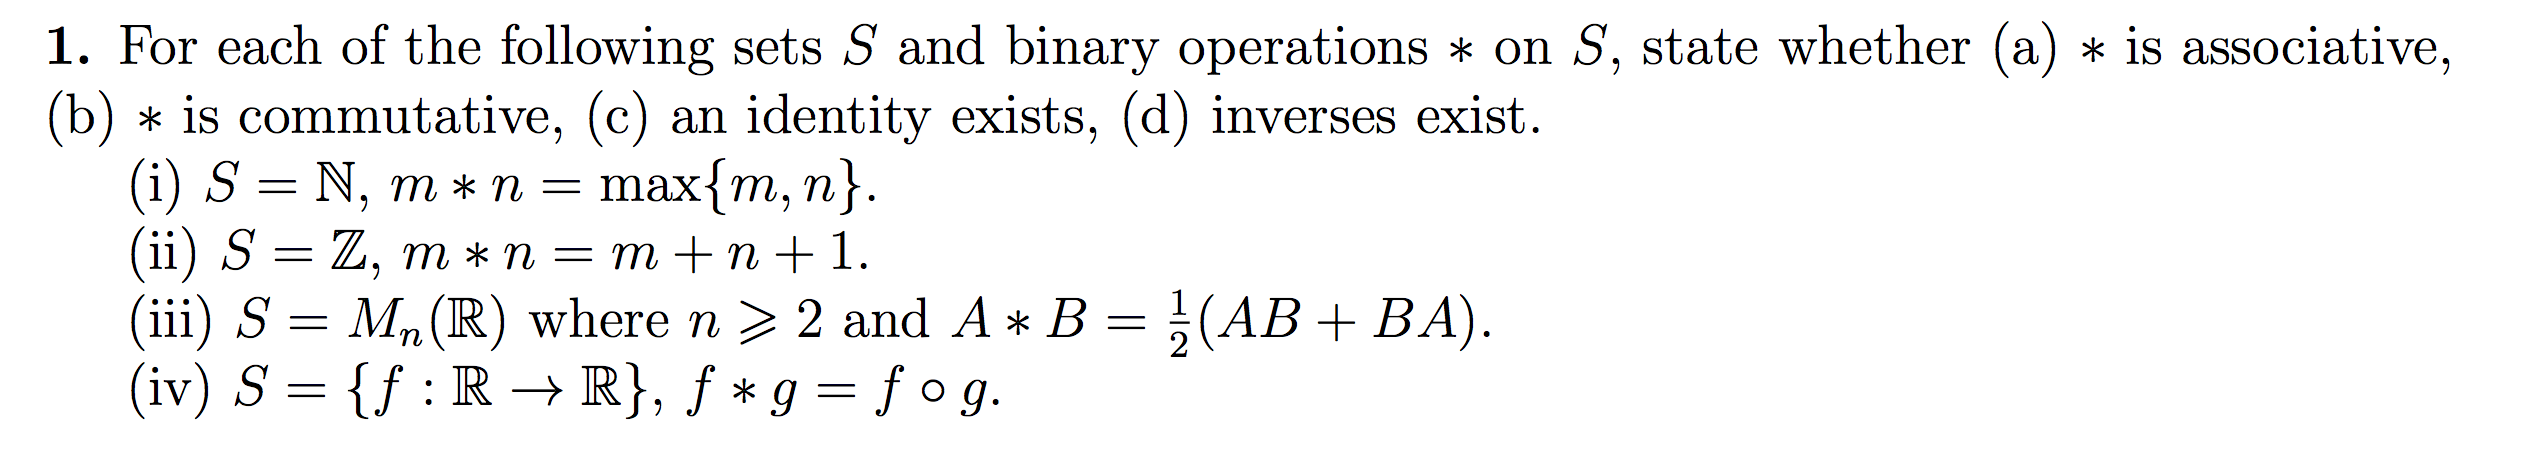
\includegraphics[width=400pt]{img/oxford-prelims-M1-groups-1-1.png}
\end{mdframed}
\begin{enumerate}[label=(\roman*)]
\item associative, commutative, identity is $e = 0$, only inverse is $e^\1 = e$.
\item associative, commutative, identity is $e = -1$, inverse is $m^\1 = -m - 2$.
\item \red{(not) associative?}, commutative, identity is $I_n$, inverse is $A^\1$\\
  Note that if $AB = BA$ then $A\cdot B = AB$, and $A\cdot(B\cdot C) = A(BC) = (AB)C$. I.e. the
  operation is associative for commutative matrices.\\

  Let $A$ be a reflection and $B$ a shear:
  $A = \matMMxNN{-1}{0}
                {0}{1}$, $B = \matMMxNN{1}{\frac{1}{\sqrt{2}}}
                                       {0}{\frac{1}{\sqrt{2}}}$.\\
  Then $AB = \matMMxNN{-1}{-\frac{1}{\sqrt{2}}}
                      {0}{~~\frac{1}{\sqrt{2}}}$ and
  and  $BA = \matMMxNN{-1}{\frac{1}{\sqrt{2}}}
                      {0}{\frac{1}{\sqrt{2}}}$,
  and $\frac{1}{2}(AB + BA) = \matMMxNN{-1}{0}
                                       {0}{\frac{1}{\sqrt{2}}}$.\\

  % E.g. let $A = I, B = 2I, C=3I$.\\
  % Then $A\cdot (B\cdot C) = I\cdot (6I)$ and $(A \cdot B)\cdot C) = 2I \cdot 3I = 6I$.
\item associative (function composition is associative), not commutative, identity is $I$, inverses
  only exist for bijections.
\end{enumerate}

\begin{mdframed}
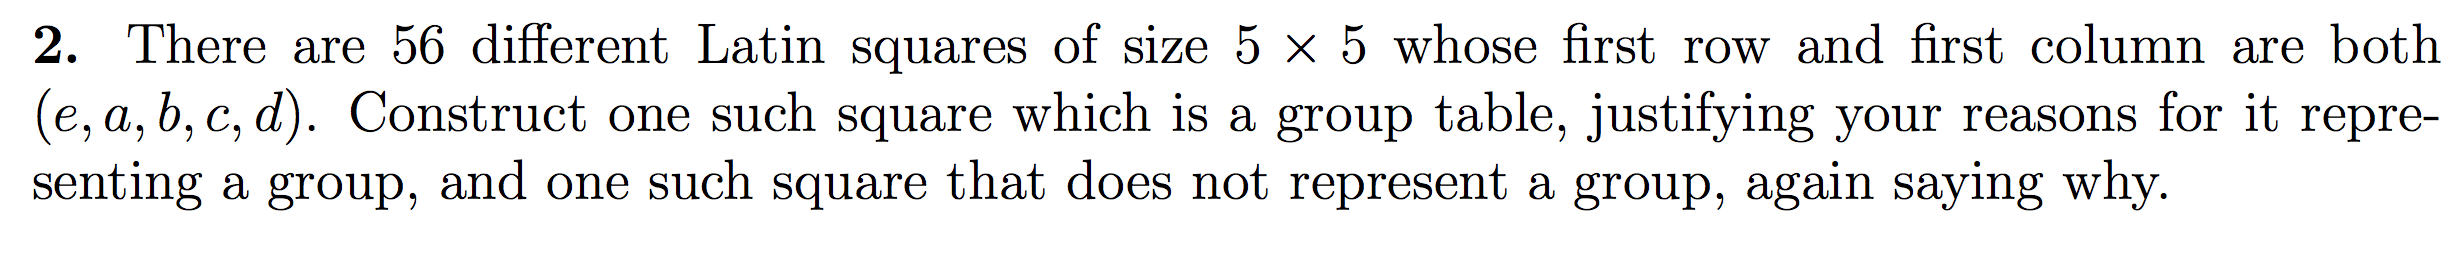
\includegraphics[width=400pt]{img/oxford-prelims-M1-groups-1-2.png}
\end{mdframed}
These both satisfy existence of identity and inverses because they are Latin squares.

Latin square, group:\\~\\
\begin{tabular}{c||c|c|c|c|c|}
    & e & a & b & c & d\\
  \hline
  \hline
  e & e & a & b & c & d\\
  a & a & b & c & d & e\\
  b & b & c & d & e & a\\
  c & c & d & e & a & b\\
  d & d & e & a & b & c
\end{tabular}\\
Group because it's isomorphic to $\Z/5\Z$.\\
Associative: e.g. $a(bc) = ae = a$ and $(ab)c = cc = a$.
Commutative.

~\\~\\
\red{Latin square, not a group:}\\~\\
\begin{tabular}{c||c|c|c|c|c|}
    & e & a & b & c & d\\
  \hline
  \hline
  e & e & a & b & c & d\\
  a & a &&&&\\
  b & b &&&&\\
  c & c &&&&\\
  d & d &&&&
\end{tabular}

\begin{mdframed}
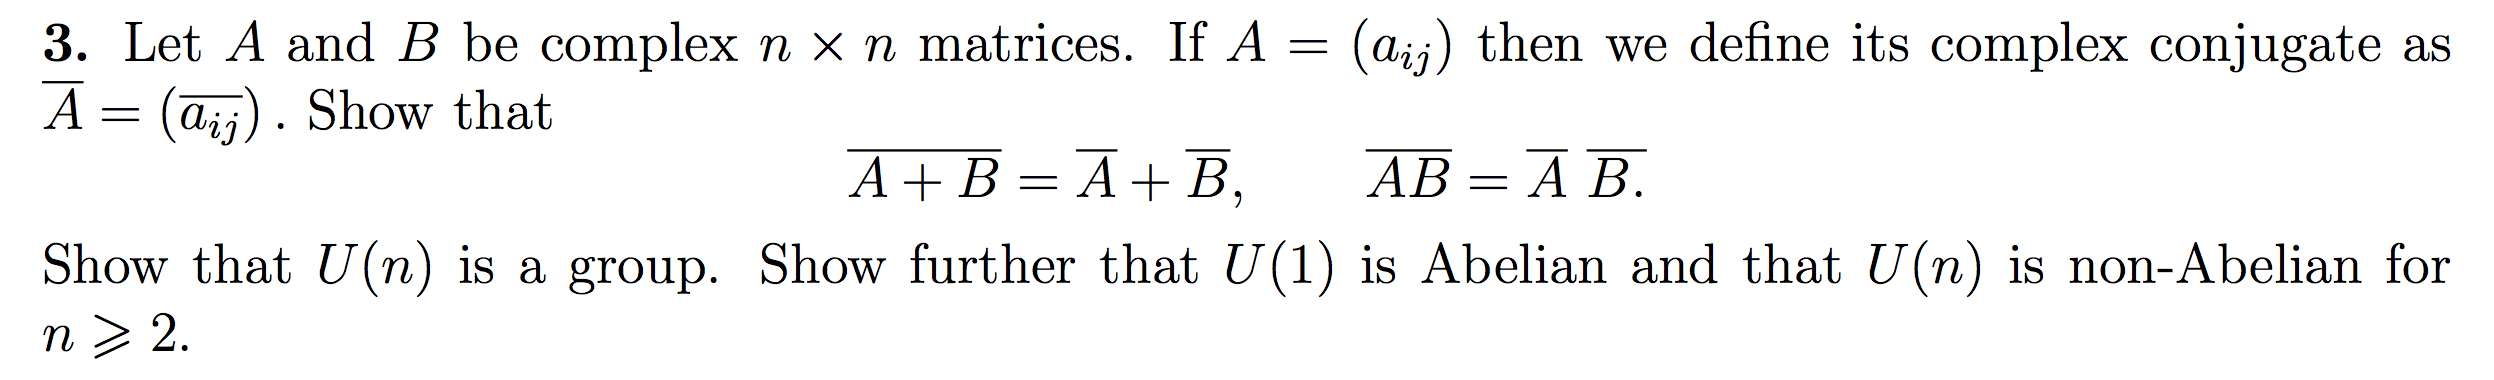
\includegraphics[width=400pt]{img/oxford-prelims-M1-groups-1-3.png}
\end{mdframed}

\begin{mdframed}
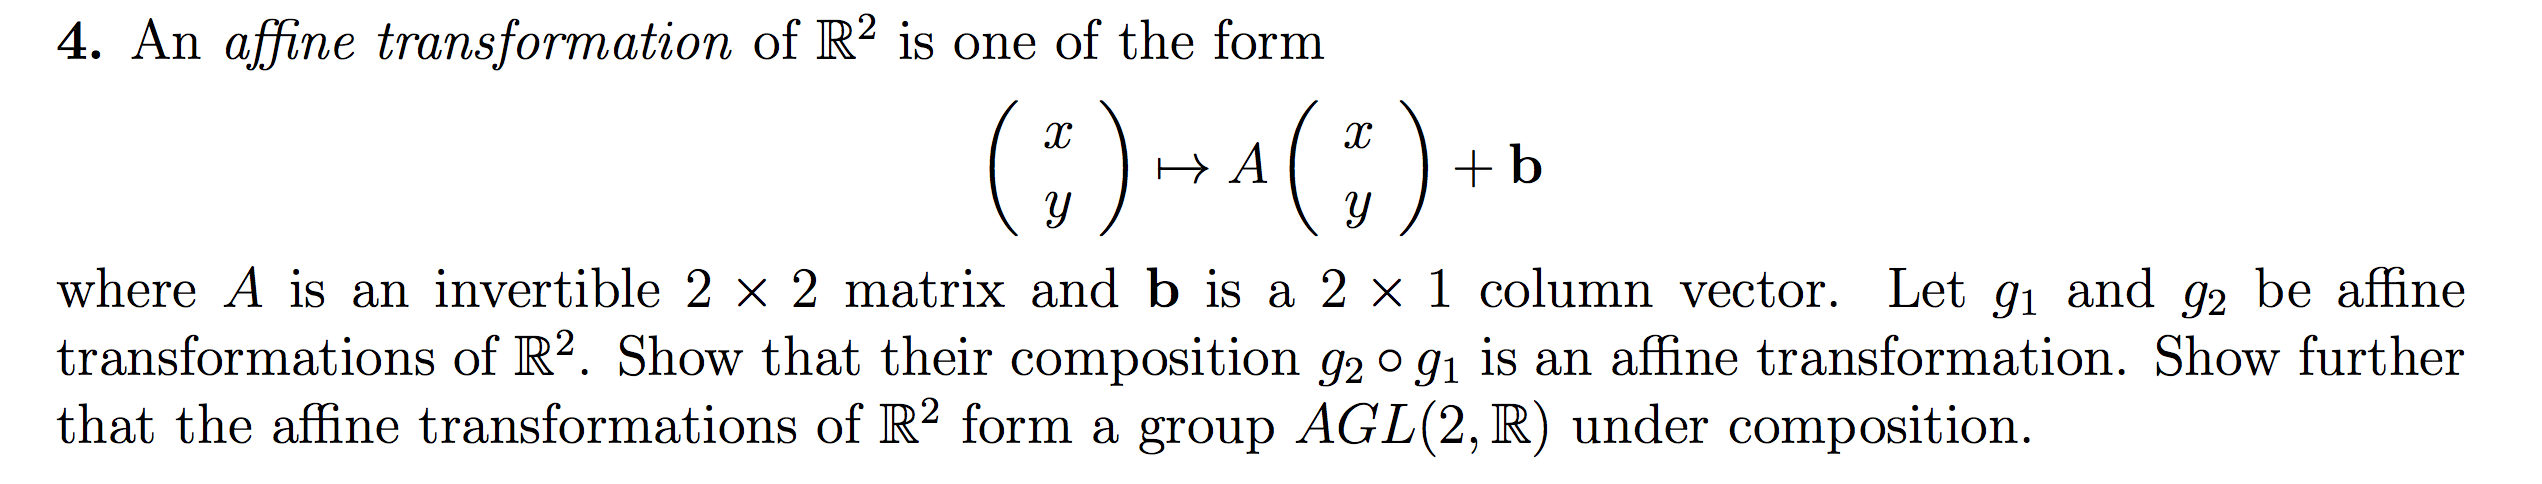
\includegraphics[width=400pt]{img/oxford-prelims-M1-groups-1-4.png}
\end{mdframed}

\begin{mdframed}
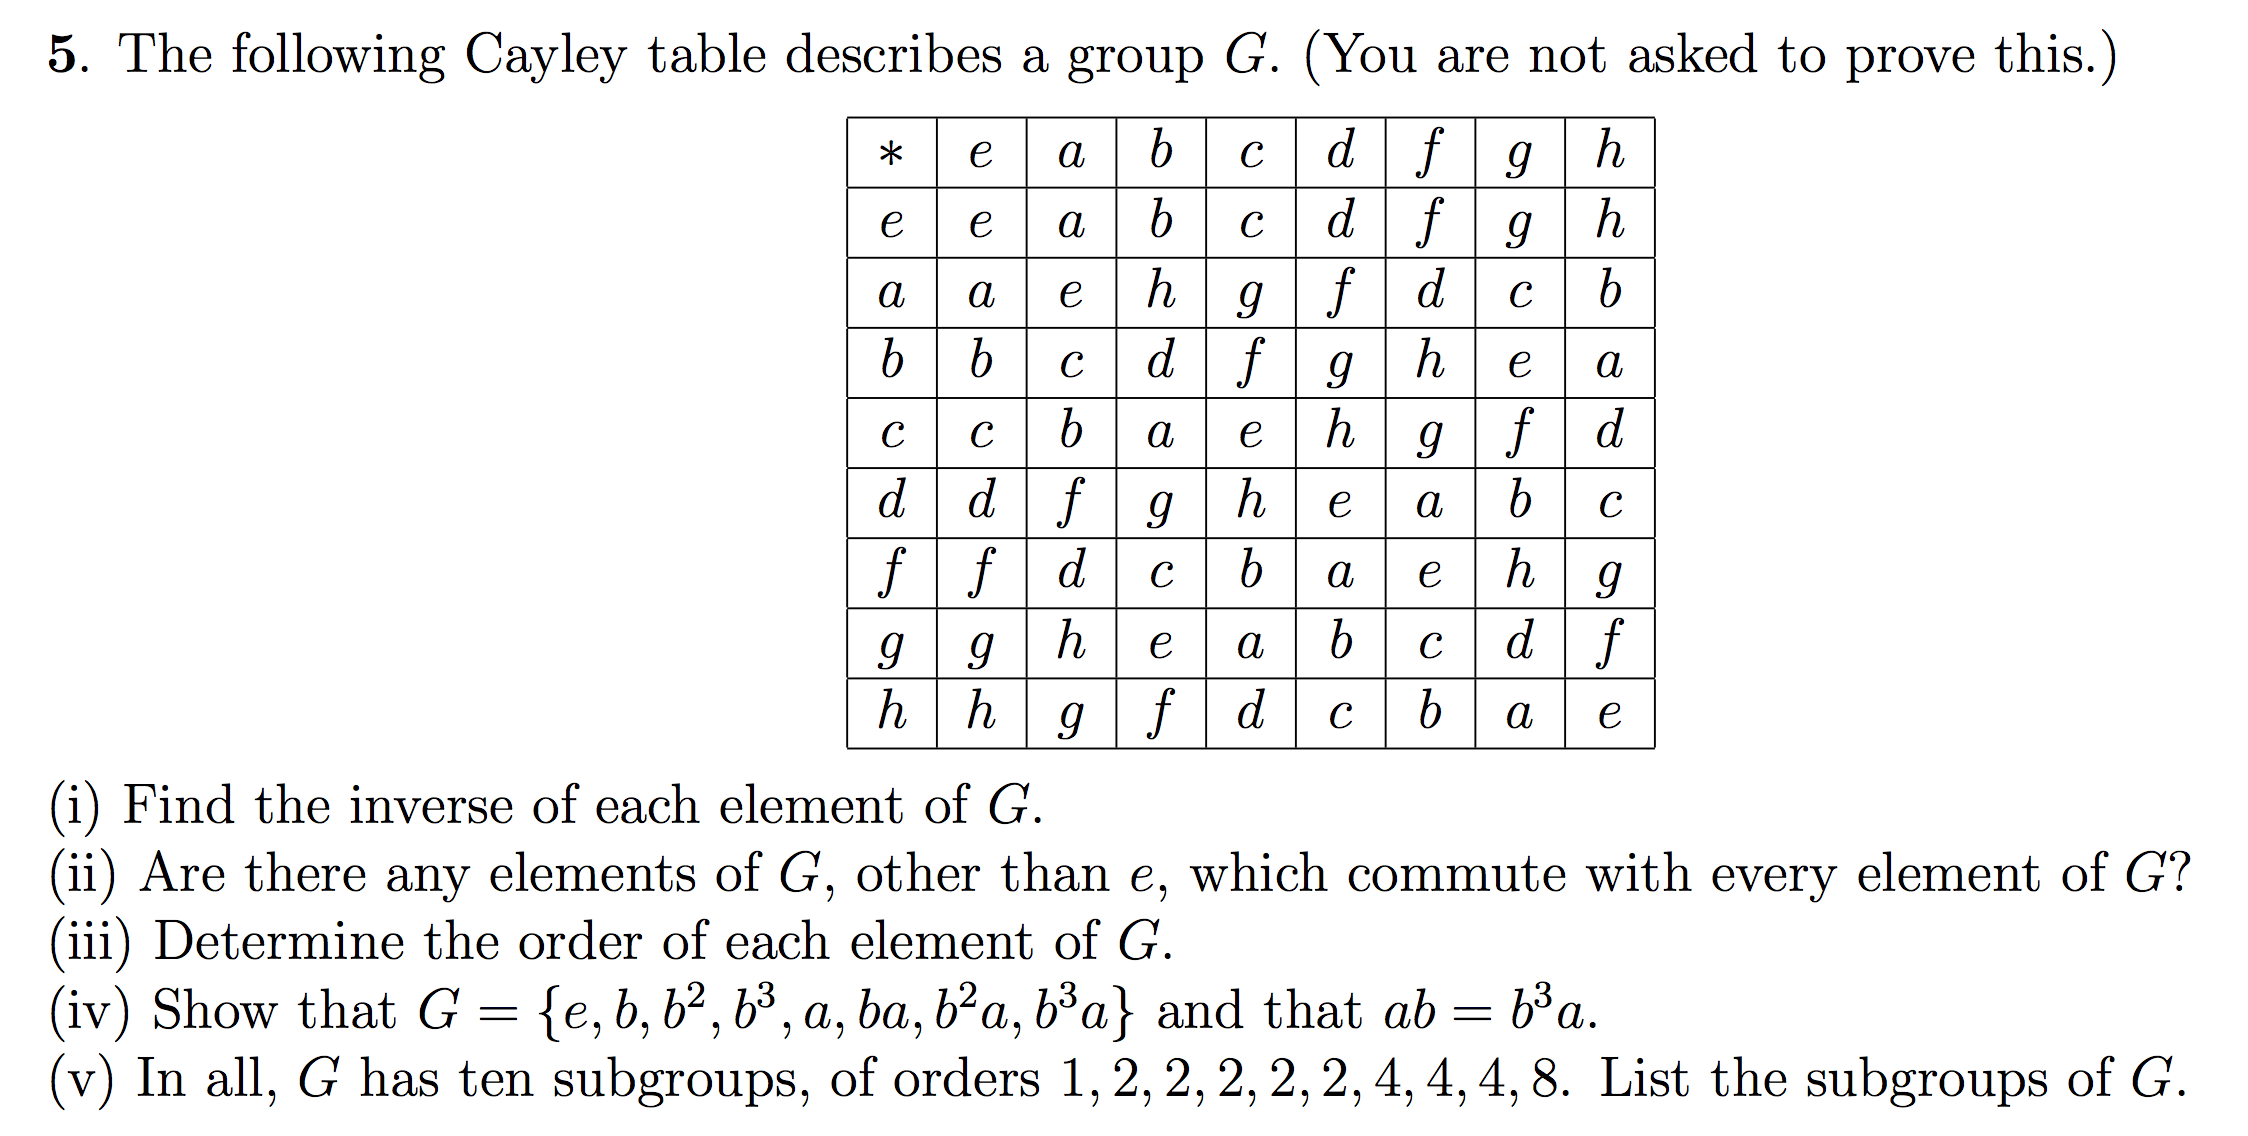
\includegraphics[width=400pt]{img/oxford-prelims-M1-groups-1-5.png}
\end{mdframed}

\begin{mdframed}
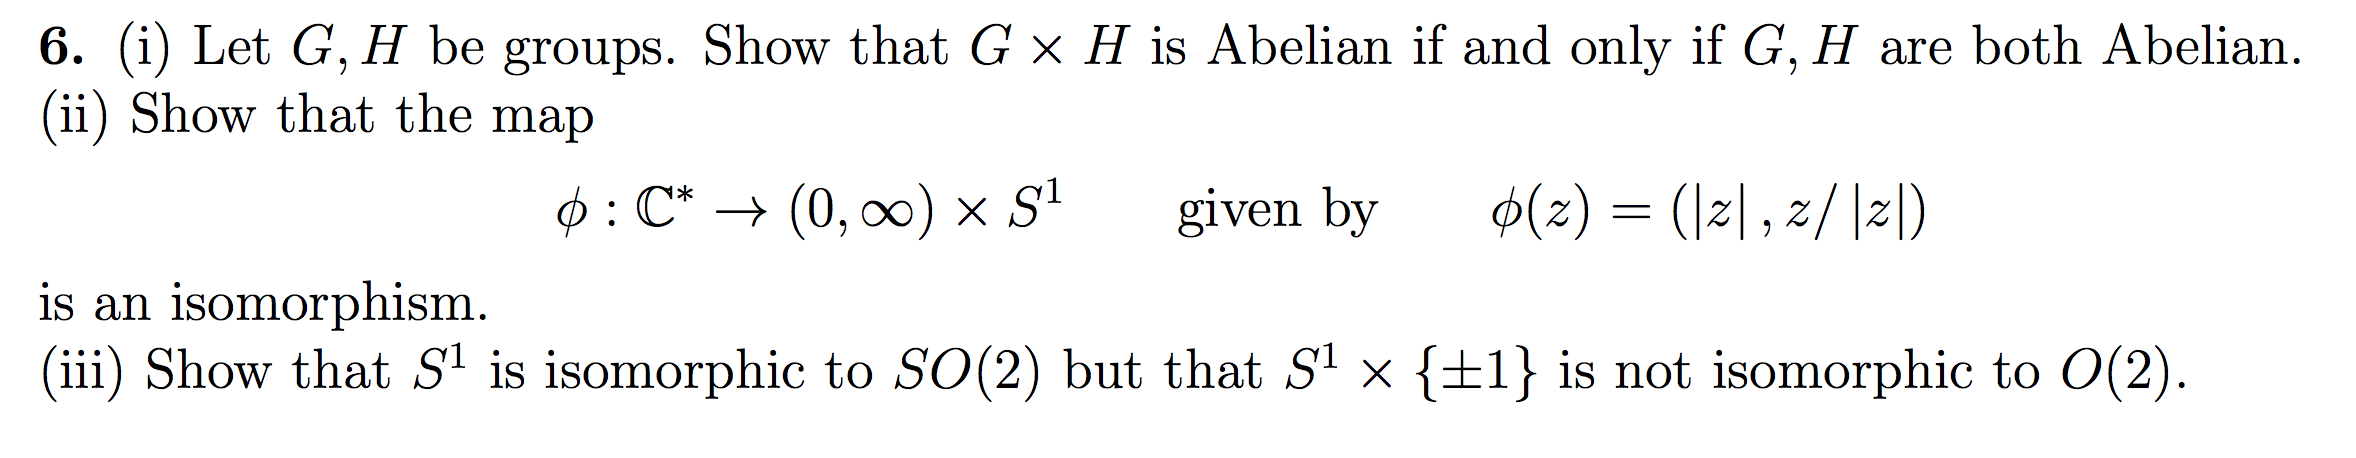
\includegraphics[width=400pt]{img/oxford-prelims-M1-groups-1-6.png}
\end{mdframed}

\newpage
\section{Sheet 5: Homomorphisms. Conjugacy. Normal Subgroups.}

\begin{mdframed}
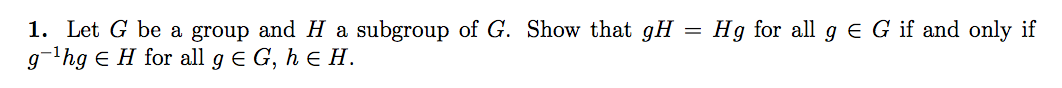
\includegraphics[width=400pt]{img/abstract-algebra-oxford-M1-5-1.png}
\end{mdframed}

\begin{claim*}
[Forwards implication]
  If $g^\1hg \in H$ for all $g \in G, h \in H$ then $gH = Hg$.
\end{claim*}

\begin{proof} We show that $Hg \subseteq gH$ and $gH \subseteq Hg$, for all $g \in G$.\\

Multiplying on the left by $g$ gives $hg \in gH$ for all $g \in G, h \in H$. Therefore $Hg \subseteq gH$ for all $g \in G$.
\end{proof}

\begin{mdframed}
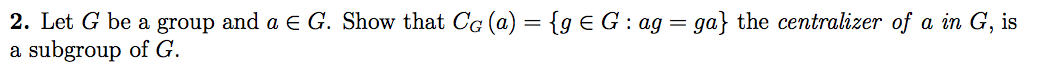
\includegraphics[width=400pt]{img/abstract-algebra-oxford-M1-5-2-1.png}
\end{mdframed}

\begin{mdframed}
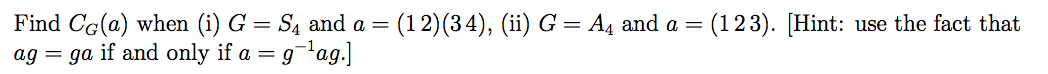
\includegraphics[width=400pt]{img/abstract-algebra-oxford-M1-5-2-2.png}
\end{mdframed}

\begin{mdframed}
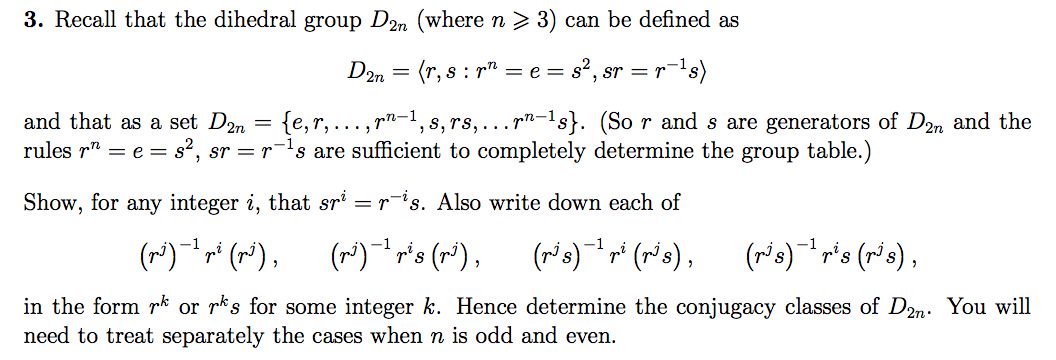
\includegraphics[width=400pt]{img/abstract-algebra-oxford-M1-5-3.png}
\end{mdframed}

\newpage
\section{Sheet 6: Quotient Groups. Isomorphism Theorem. Group Actions.}

\begin{mdframed}
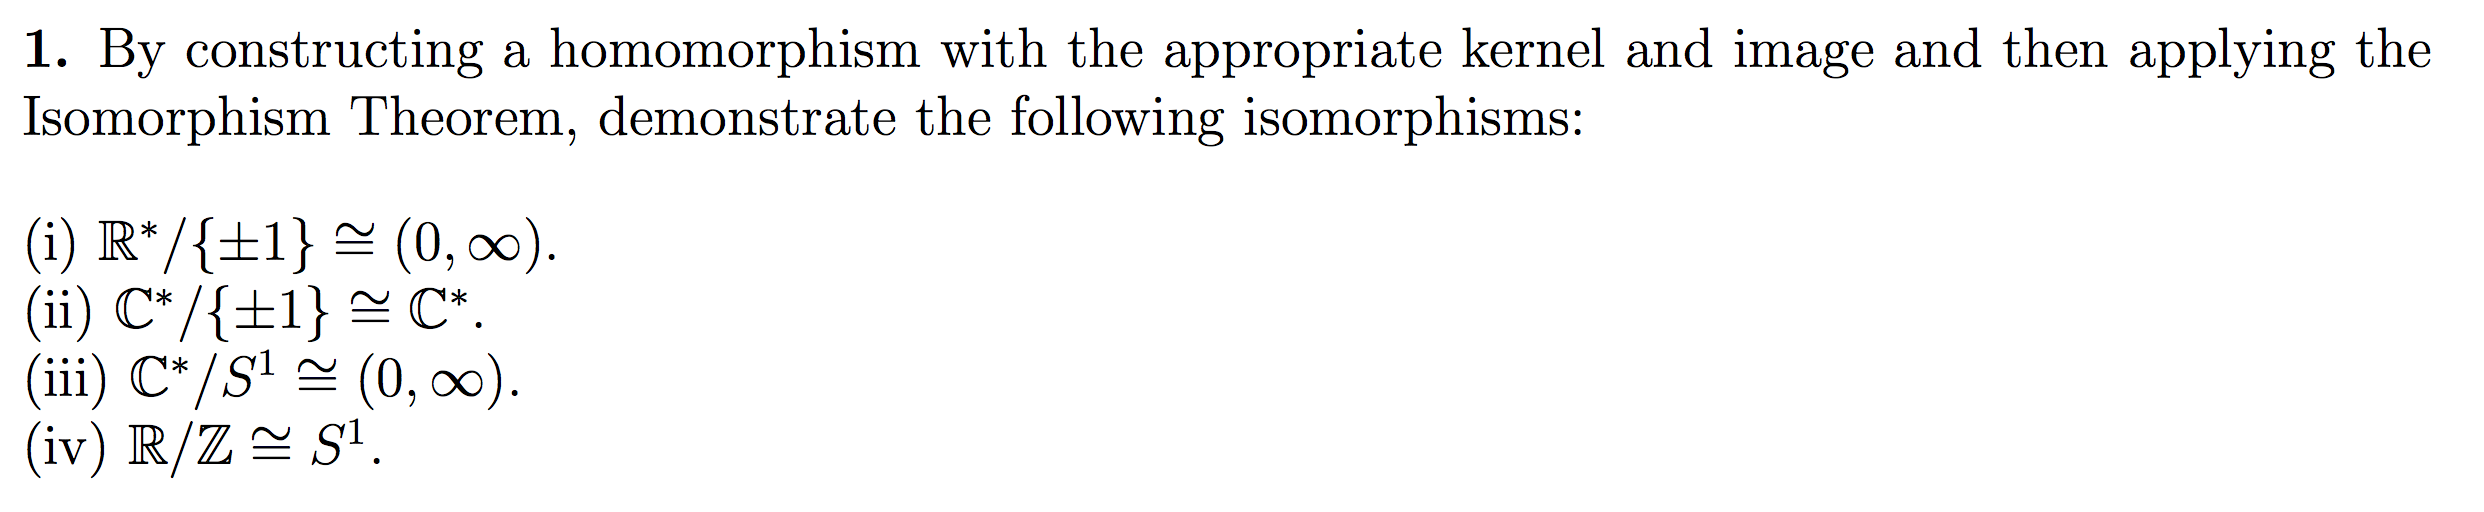
\includegraphics[width=400pt]{img/abstract-algebra-oxford-M1-6-1.png}
\end{mdframed}

\begin{theorem*}[First Isomorphism Theorem]~\\
  Let $\varphi:G_1 \to G_2$ and let $H$ be the kernel of $\varphi$. Then
  \begin{enumerate}
  \item $\Im \varphi \cong G/ \ker \varphi$
  \end{enumerate}
\end{theorem*}

\subsection*{(i): $\R^*/\{\pm 1\} \cong (0, \infty)$}

We have a group $G = \R^* = \R\setminus\{0\}$.

We have a subgroup $H = \{\pm 1\}$.

The group is abelian hence the subgroup is normal.

The set of cosets is $G/H = \{(0, \infty), (-\infty, 0)\}$.

Define the homomorphism $\varphi: G \to G/H$.

The image of $\varphi$ is the set of cosets $G/H$.

The kernel of $\varphi$ is $(0, \infty)$.

\end{document}
